\chapter{MAKE : Graphical Error Modelling} % Chapter title
%
\label{ch:graph}	
	
	Here we extend our proposed split-up heuristics to graphical error models or the algorithm MAKE.
	The motivation behind this creation of MAKE is to aid the identification and suggestion of solutions to the most probabilistic errors.
	For example, there are many common errors in the spelling typographical errors, like: \textit{ie} is commonly mistaken with \textit{ei}, adding or deleting of an extra \textit{l} in \textit{lly} and so on.
	
	\begin{algorithm}
		\caption{MAKE algorithm}\label{point}
		\begin{algorithmic}[1]
			\Procedure{MAKE($first, second$)}{}
			
			\If{$first.size = 0$}
			\State $first.insert(\phi)$
			\EndIf
			
			\If{$second.size = 0$}
			\State $second.insert(\phi)$
			\EndIf
			
			\While{$first.size < second.size$}
			\State $position \gets \left \lceil{\frac{first.size}{2}}\right \rceil $
			\State $first.insert(\phi, position)$
			\EndWhile
			
			\While{$first.size > second.size$}
			\State $position \gets \left \lfloor{\frac{second.size}{2}}\right \rfloor $
			\State $second.insert(\phi, position)$
			\EndWhile
			
			\State $graph = \lbrace \rbrace$
			
			\For{$i\gets 0, first.size$}
			\State $map\gets pair(first[i], second[i])$
			\State $graph.insert(map)$
			\EndFor
			
			\For{$i\gets 0, first.size - 1$}
			\State $map\gets pair(first[i], second[i + 1])$
			\State $graph.insert(map)$
			\EndFor
			
			\For{$i\gets 1, first.size$}
			\State $map\gets pair(first[i], second[i - 1])$
			\State $graph.insert(map)$
			\EndFor
			
			\State $graph.remove\_duplicates()$
			\State \textbf{return} $graph$
			\EndProcedure
		\end{algorithmic}
	\end{algorithm}
	
	
	The algorithm \ref{point} process of MAKE.
	Let $Q$ be the query and $D$ be the document.
	Thus $Q \cap D$ shows number of terms common between them.
	We are interested in the leftover terms in the sets.
	That means, we need to infer a certain pattern from leftover sets, which are $Q - \lbrace Q \cap D \rbrace$ and $D - \lbrace Q \cap D \rbrace$.
	Thus we can draw mappings to gather information of the corrections.
	
	
	
	Let \textit{first} and \textit{second} be the \textbf{ordered sets} referring to $Q - \lbrace Q \cap D \rbrace$ and $D - \lbrace Q \cap D \rbrace$ respectively.
	If \textit{first} or \textit{second} are empty, then we insert empty token $\phi$ in them (Lines 2-5 of the algorithm).
	
	
	If size of \textit{first} is less than size of the \textit{second}, then we keep inserting empty tokens $\phi$ in the middle of \textit{first}, unless the size of \textit{first} becomes equal to the size of \textit{second} (Lines 6-8).
	Similarly, if the size of \textit{second} is less than size of the \textit{first}, then we keep inserting empty tokens $\phi$ in the middle of \textit{second}, unless the size of \textit{second} becomes equal to the size of \textit{first} (Lines 9-11).
	
	We now initialize a hash map \textit{graph} (Line 12).
	We make pairs from the members of the \textit{first} which corresponds to the \textit{second} and insert in the \textit{graph}.
	We insert pairs of the corresponding same index of \textit{first} and \textit{second} in the \textit{graph} (Lines 13-15).
	We then insert pairs of the corresponding indexes of \textit{first} and \textit{second} in the \textit{graph}, with one index ahead of others (Lines 16-18).
	In the same way, we insert pairs of the corresponding indexes of \textit{first} and \textit{second} in the \textit{graph}, with one index before others (Lines 19-21).
	
	After removing the duplicates, we can return the graph as a result. Following example shows the procedure of the algorithm.
	
	\textbf{Example 1, Deletion error:} We will visualize \textit{pizza} again. 
	Let the correct split-set of \textit{pizza} (ignoring the offsets) be $D$, which is indexed in the document.
	So, $D = \left\lbrace \textit{1p, 2pi, 3iz, zz3, za2, a1} \right\rbrace$.
	Let the incorrect split-set of \textit{piza} (ignoring the offsets) be $Q$ given as the query.
	So, $Q = \left\lbrace \textit{1p, 2pi, 3iz, za2, a1} \right\rbrace$.
	Thus the term matches are, 
	$Q \cap D = \left\lbrace \textit{1p, 2pi, 3iz, za2, a1} \right\rbrace$.
	
	Now we can analyze the leftover \textit{pizza} sets, which are $D - Q \cap D$ (\textit{first}) and $Q - Q \cap D$ (\textit{second}).
	Hence, $Q - Q \cap D = \left\lbrace \textit{zz3} \right\rbrace$
	Similarly, $D - Q \cap D = \left\lbrace \phi \right\rbrace$
	
	Graph is now constructed from the members of $D - Q \cap D$ to $Q - Q \cap D$.
	The graph constructed is $\left\lbrace \phi \rightarrow \textit{zz3} \right\rbrace$.
	
	Intuitively, $\phi \rightarrow \textit{zz3}$ means that the letter \textit{z} should have been inserted around position 3 from the last.
	
	The query set $Q$, is mentioned here as $I$, which means incorrect split-set and the document set $D$, is mentioned here as $C$, which means the correct split set.
	
	\textbf{Example 2, Insertion error:} For the misspelled word \textit{pizzza}, we have:
	\begin{equation*}
	\begin{aligned}
	C &= \left\lbrace \textit{1p, 2pi, 3iz, zz3, za2, a1} \right\rbrace \\
	I &= \left\lbrace \textit{1p, 2pi, 3iz, 4zz, zz3, za2, a1} \right\rbrace \\
	C \cap I &= \left\lbrace \textit{1p, 2pi, 3iz, zz3, za2, a1} \right\rbrace \\
	C - C \cap I &= \left\lbrace \phi \right\rbrace \\
	I - C \cap I &= \left\lbrace \textit{4zz} \right\rbrace 
	\end{aligned}
	\end{equation*}
	
	Thus the graph constructed is, $\left\lbrace \textit{4zz} \rightarrow  \phi \right\rbrace$.
	Intuitively, $\textit{4zz} \rightarrow  \phi$ means that the letter \textit{z} starting around 4th position should have been deleted.
	
	\textbf{Example 3, Substitution error:} For the misspelled word \textit{panc} and the correct word \textit{pant}, we have:
	\begin{equation*}
	\begin{aligned}
	C &= \left\lbrace \textit{1p, 2pa, 3an, nt2, t1} \right\rbrace \\
	I &= \left\lbrace \textit{1p, 2pa, 3an, nc2, c1} \right\rbrace \\
	C \cap I &= \left\lbrace \textit{1p, 2pa, 3an} \right\rbrace \\
	C - C \cap I &= \left\lbrace \textit{nt2, t1} \right\rbrace \\
	I - C \cap I &= \left\lbrace \textit{nc2, c1} \right\rbrace
	\end{aligned}
	\end{equation*}
	\begin{figure}[h]
		\centering
		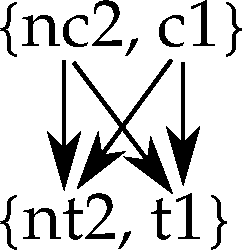
\includegraphics[width=0.35\textwidth]{gfx/ex3.pdf}
		\caption{Graphical error model construction from \textit{panc} to \textit{pant}}
		\label{e3}
	\end{figure}
	
	The figure \ref{e3} clearly shows the set mappings done by the for loop. They correspond to the same index, one index ahead and one index behind from the first set to the second set.
	
	Thus the graph constructed is, $\left\lbrace \textit{nc2} \rightarrow  \textit{nt2}, \textit{nc2} \rightarrow  \textit{t1}, \textit{c1} \rightarrow  \textit{nt2}, \textit{c1} \rightarrow  \textit{t1} \right\rbrace$.
	Intuitively, this graph depicts that the last letter should have been \textit{t}.
	
	\textbf{Example 4, Swapping error:} For the misspelled word \textit{sieze} and the correct word \textit{seize}, we have:
	\begin{equation*}
	\begin{aligned}
	C &= \left\lbrace \textit{1s, 2se, 3ei, iz3, ze2, e1} \right\rbrace \\
	I &= \left\lbrace \textit{1s, 2si, 3ie, ez3, ze2, e1} \right\rbrace \\
	C \cap I &= \left\lbrace \textit{1s, ze2, e1} \right\rbrace \\
	C - C \cap I &= \left\lbrace \textit{2se, 3ei, iz3} \right\rbrace \\
	I - C \cap I &= \left\lbrace \textit{2si, 3ie, ez3} \right\rbrace
	\end{aligned}
	\end{equation*}
	\begin{figure}[h]
		\centering
		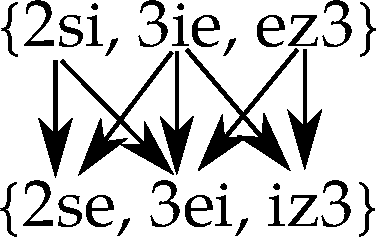
\includegraphics[width=0.5\textwidth]{gfx/ex4.pdf}
		\caption{Graphical error model construction from \textit{sieze} to \textit{seize}}
		\label{e4}
	\end{figure}
	
	Thus the graph constructed is, $\lbrace \textit{2si} \rightarrow  \textit{2se}, \textit{2si} \rightarrow  \textit{3ei}, \textit{3ie} \rightarrow  \textit{2se}, \textit{3ie} \rightarrow  \textit{3ei},$ $ \textit{3ie} \rightarrow  \textit{iz3}, \textit{ez3} \rightarrow  \textit{3ei}, \textit{ez3} \rightarrow  \textit{iz3} \rbrace$.
	Thus the graph neatly captures the idea that the letters \textit{i} and \textit{e} should have been swapped.
	
	\textbf{Example 5, Unequal set length:} For the misspelled word \textit{pth} and the correct word \textit{path}, we have:
	\begin{equation*}
	\begin{aligned}
	C &= \left\lbrace \textit{1p, 2pa, 3at, th2, h1} \right\rbrace \\
	I &= \left\lbrace \textit{1p, 2pt, th2, h1} \right\rbrace \\
	C \cap I &= \left\lbrace \textit{1p, th2, h1} \right\rbrace \\
	C - C \cap I &= \left\lbrace \textit{2pa, 3at, th2} \right\rbrace \\
	I - C \cap I &= \left\lbrace \textit{2pt} \right\rbrace
	\end{aligned}
	\end{equation*}
	\begin{figure}[h]
		\centering
		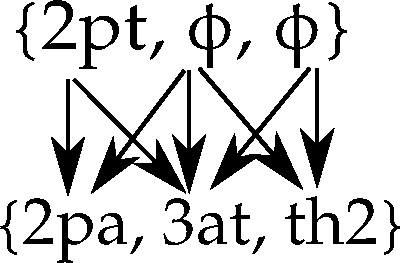
\includegraphics[width=0.5\textwidth]{gfx/ex5.pdf}
		\caption{Directed graph guiding from the incorrect \textit{pth} to the correct \textit{path}}
		\label{e5}
	\end{figure}
	
	Since the size of topmost set was not equal to the bottom one, we inserted empty tokens in the top one unless they become of equal sizes.
	Thus the graph constructed is, $\lbrace \textit{2pt} \rightarrow  \textit{2pa}, \textit{2pt} \rightarrow  \textit{3at}, \phi \rightarrow  \textit{2pa}, \phi \rightarrow  \textit{3at} \rbrace$.
	Thus the graph roughly conveys the information that the letter \textit{t} should be second last.
	
	\textbf{Example 6, Unequal set length:} For the misspelled word \textit{patthhs} and the correct word \textit{paths}, we have:
	\begin{equation*}
	\begin{aligned}
	C &= \left\lbrace \textit{1p, 2pa, 3at, th3, hs2, s1} \right\rbrace \\
	I &= \left\lbrace \textit{1p, 2pa, 3at, 4tt, th4, hh3, hs2, s1} \right\rbrace \\
	C \cap I &= \left\lbrace \textit{1p, 2pa, 3at, hs2, s1} \right\rbrace \\
	C - C \cap I &= \left\lbrace \textit{th3} \right\rbrace \\
	I - C \cap I &= \left\lbrace \textit{4tt, th4, hh3} \right\rbrace
	\end{aligned}
	\end{equation*}
	\begin{figure}[h]
		\centering
		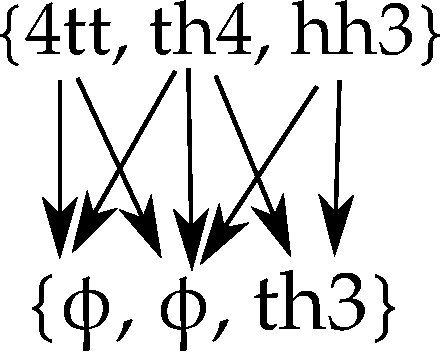
\includegraphics[width=0.5\textwidth]{gfx/ex7.pdf}
		\caption{Graphical error model construction}
		\label{e6}
	\end{figure}
	
	Since the size of bottom set was not equal to the top one, we inserted empty tokens in the bottom set at the middle, unless they become of equal sizes.
	Thus the graph constructed is, $\lbrace \textit{4tt} \rightarrow  \phi, \textit{th4} \rightarrow  \phi, \textit{th4} \rightarrow  \textit{th3}, \textit{hh3} \rightarrow  \phi,  \textit{hh3} \rightarrow  \textit{th3} \rbrace$.
	Thus the graph roughly conveys the information that the letter \textit{t} and letter \textit{h} should have been deleted.
	
	
	In order to evaluate the efficiency of the graphical error model, we will add the probability of each edge of the graph to the score of the ranking function.
	In other words, this would be:
	\begin{equation*}
	\textit{score}(q, d) =  \lambda \times \textit{rank(q, d)} + (1 - \lambda) \times \pi \textit{(q, d)}
	\end{equation*}
	where, $\lambda$ is the weight ranging from $[0, 1]$, \textit{score(q, d)} is the similarity scoring function like BM25 \cite{bm25} or Dirichlet \cite{dirich}  and $\pi \textit{(q, d)}$ is the probabilistic estimate of given error occurring in the training data.
	\begin{equation*}
	\begin{aligned}
	\pi \textit{(q, d)} =  \sum_{g \in G} \textit{count(g)}^s
	\end{aligned}
	\end{equation*}
	Here, $G$ is the constructed graph and $s$ is the strength parameter.
	\textit{count(g)} is the frequency of the error in whole training set of spelling errors.
	We have used $s$ here, to avoid the overfitting during the training, since \textit{count(p)} could heavily depend on the training data.
	
	This function can also be normalized with respect to the cardinality of the pointer set. 
	This could be useful since some of the extremely irrelevant incorrect matches would contain a lot of zeros.
	Thus normalization version, could avoid the skewness of the frequencies.
	
	The normalized version or MAKE is:
	\begin{equation*}
	\begin{aligned}
	\pi \textit{(q, d)} =  \frac{1}{|G|} \sum_{g \in G} \textit{count(g)}^s
	\end{aligned}
	\end{equation*}